%
% Chapter 10
%

\chapter{SYSTEMATIC UNCERTAINTIES}
Systematic uncertainties, often referred to as simply ``systematics'' arise from the uncertainty related to specific components of the signal
and background predictions. These components are categorized as theoretical uncertainties associated with MC event generators, scale factor uncertainties
related to data and MC yields, and uncertainties arising from control regions for data-driven background estimations.  

Systematic uncertainties are accounted for in the maximum likelihood fit in the form of nuisance parameters. Each nuisance represents a systematic uncertainty
and affects either the overall normalization of the discriminant, known as a rate uncertainty, or the shape of the discriminant,
known as a shape uncertainty\footnote{Some shape systematics also vary the overall normalization}. The rate uncertainty scales all bins of the discriminant
by a constant factor, while the shape uncertainty varies individual bins separately, thus changing the shape of the discriminant.
The rate uncertainties use a log-normal prior, while the shape uncertainties use a gaussian prior. 

The correlations, or lack thereof, of each of the 212 nuisances in this analysis are accounted for in the likelihood fit. 
Rate uncertainties arising from the same source, are treated as fully correlated across event categories. Shape uncertainties are fully correlated between
bins of the discrmininant in each category. The bin-by-bin shape uncertainties, which account for limitied statistics, are treated as uncorrelated. 


\section{Theoretical Uncertainties}
The theoretical uncertainties in this analysis arise from the NLO calculation of the cross section for the signal and background processes.
All theoretical uncertainties propagated as into the fit as rate uncertainties. For \tth signal,
these uncertainties amount to +5.8$\%$ -9.2$\%$ from unknown higher order terms in the perturbative expansion and an additional 3.6$\%$ uncertainty for the
PDFs and the scale ($\alpha_{s}$). For the leading MC background of \ttw and \ttz, the cross section uncertainties are 12$\%$ and 10$\%$ respectively, with
scale uncertainties of 2$\%$ and 3$\%$ respectively~\cite{xsec_uncert}. A conservative 50$\%$ uncertainty is assigned to all other background MC processes. 


\section{Scale Factor Uncertainties}
\section{Data-driven Background Uncertainties}






%% \begin{figure}[hbtp]
%%  \begin{center}
%%    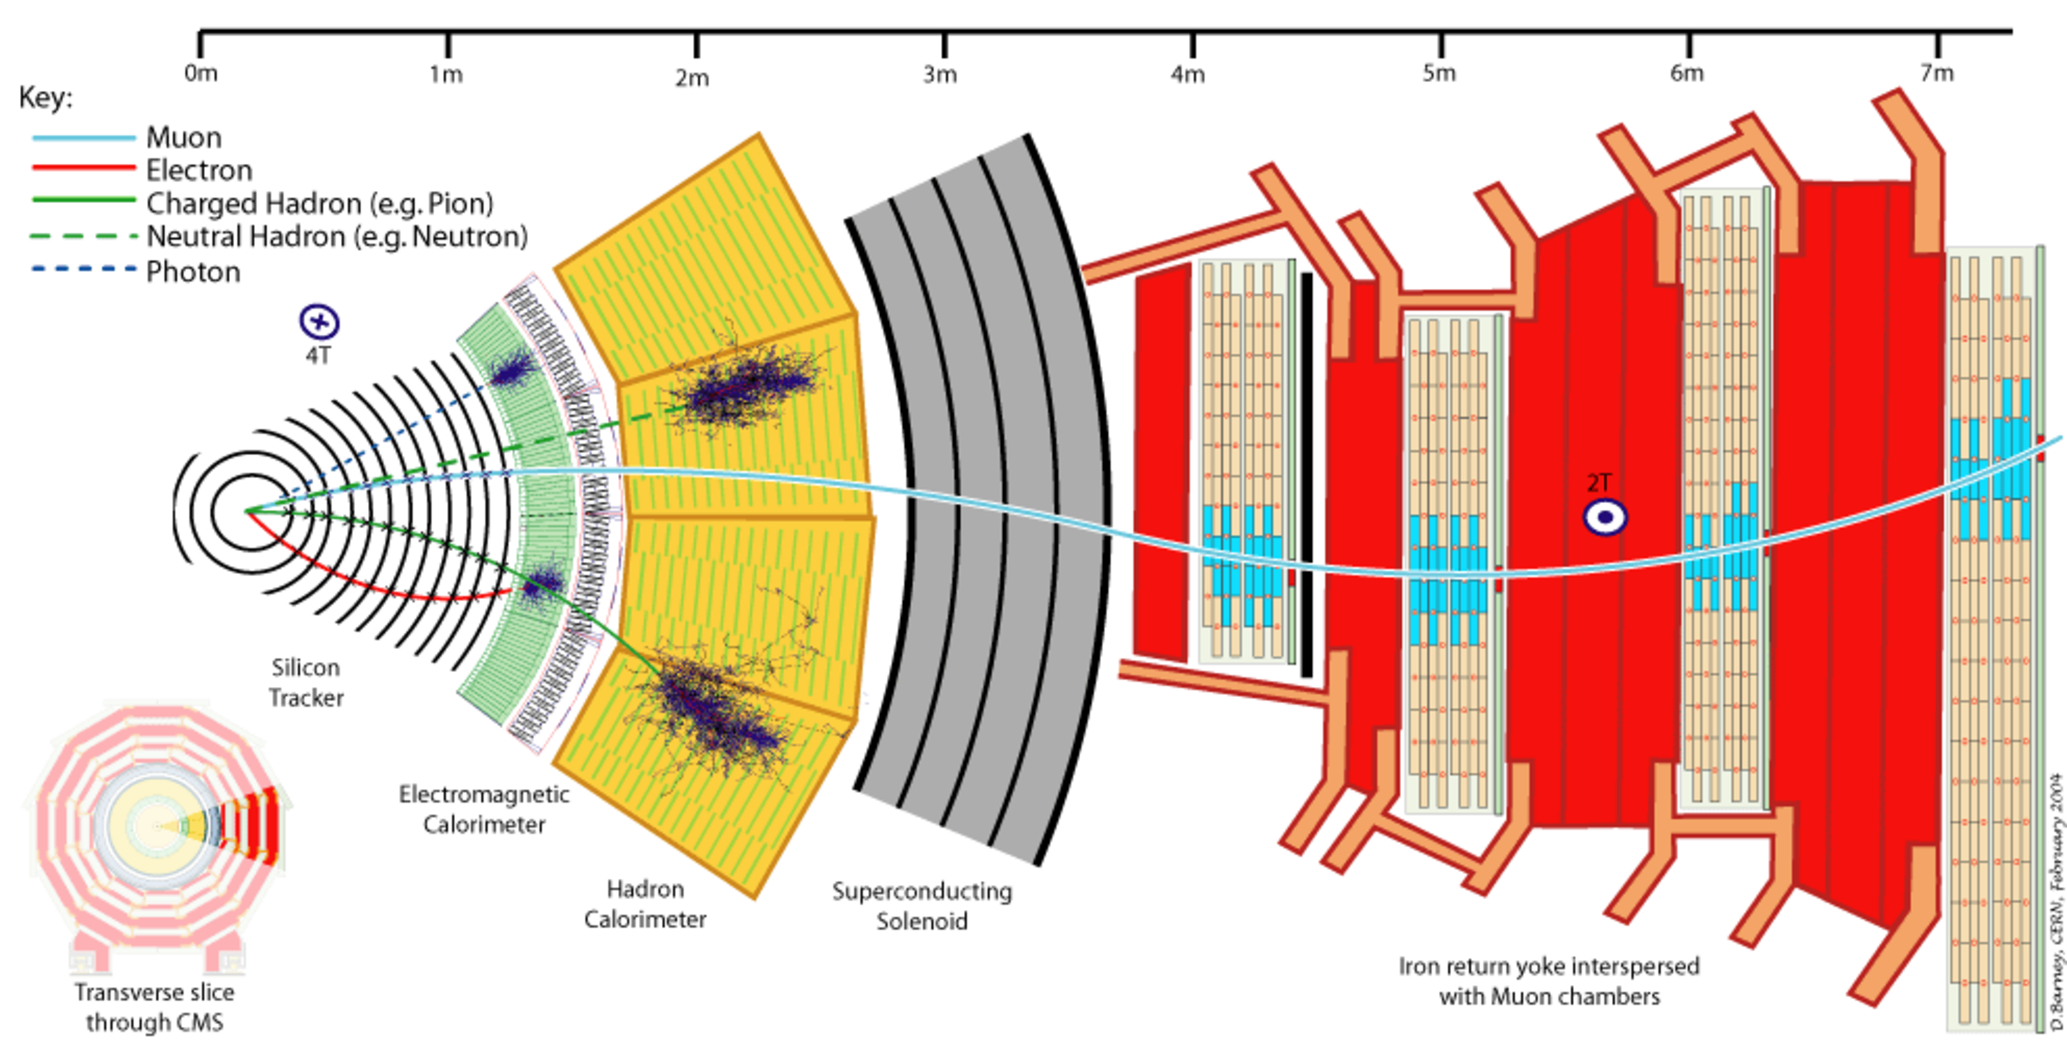
\includegraphics[width=0.8\textwidth]{ch4_figs/cms_particleflow.pdf}
%%    \caption{An overview of how CMS detects different types of particles. The slice of CMS in in the x-y plane.~\cite{NEED CITATION}.}
%%    \label{fig:cms_pflow}
%%  \end{center}
%% \end{figure}
